\documentclass{article}
\usepackage[margin=1in]{geometry}
\usepackage{mathtools, amsfonts, amsthm, xcolor, listings}

\newcommand{\R}{\mathbb{R}}
\newcommand{\N}{\mathbb{N}}
\newcommand{\I}{\mathbb{I}}
\newcommand{\Q}{\mathbb{Q}}
\newcommand{\Z}{\mathbb{Z}}

\newcommand{\set}[1]{\left\{#1\right\}}
\newcommand{\ang}[1]{\left\langle #1 \right\rangle}
\newcommand{\inv}{^{-1}}

\newcommand{\normsub}{\lhd}

\newcommand{\reflection}[5]{
    \begin{itemize}
    \item Points attempted: #1
    \item Self-assessed score: #2/#1.
    \item Time spent: #3 minutes.
    \item Difficulty: #4/10.
    \item Questions/Feedback: #5.
    \end{itemize}
}


\title{HW07}
\author{Sam Ly}

\begin{document}
\maketitle

\section*{Exercise 2}
\begin{itemize}
  \item Points attempted: 5
  \item Self-assessed score: 5/5.
  \item Time spent: 60 minutes.
  \item Difficulty: 6/10.
  \item Questions/Feedback: Clarity, correctness.
\end{itemize}
\begin{enumerate}
    \item {
        [2] Read Tai-Danae Bradley's blog post What's a Quotient Group, Really? Part 1. (Professor Bradley wrote this blog when she was in graduate school, and her blog was a part of the motivation for doing a blog post as the term paper in this class.)

        Done.
    }
    \item {
        HW7, Exercise 2: i added the defintion of an abelian group.
    }

    \item {
        Do at least \emph{three} of the following for your blog:

        \begin{enumerate}
            \item[a] {
                Write an outline of what your blog post is going to be about.

                Although the full prompt that I will be folllowing is ``The 
                Fundamental Group of a Topological Space'', I want to maybe open 
                up the scope just a tad, and include more details about algebraic 
                topology itself. Thus, I want to include a section on specifically 
                the foundations of algebraic topology. Then, as a we build solid 
                foundation, the blog should transition into a more focused discussion 
                about how groups show up in algebraic topology, specifically as 
                the fundamental group of a topological space.

                Lastly, I want to also get into some applications. As I am 
                currently deeply interested in machine learning, and the 
                mathematical foundations of it, I want to explore some applications 
                of topology in machine learning. There is also a concept in 
                deep learning known as the \textbf{manifold hypothesis} which 
                states that `most' high dimensional data can actually be summarized 
                as a manifold with a lower `intrinsic dimensionality.'
            }
            \item[b] {
                Write two paragraphs explaining a core concept or idea.

                The bedrock of topology is a concept known as \textbf{homotopy}.
                Although topology is often introduced in terms of donuts and mugs, 
                I believe that a slightly more `formal' defintion is worth investing 
                into before we continue.
                Without too much detail[TK], suppose we have two topological spaces 
                \(X\) and \(Y\). Now, consider two maps from \(f, f' \colon X \to Y\).
                We consider \(f\) and \(f'\) \textbf{homotopic} if we can ``continuously
                deform'' one into the other. This may be hard to visualize, but 
                imagine that we have two topological spaces, one that is the 
                perimeter of a circle, and another that is the perimeter of a 
                square, (we will see later that these two are inherently the 
                same space, but for now, we can treat them as different spaces).
                Notice that all mappings from a circle to a square can be
                be deformed into each other, if they have a specific quality:
                that they go around the object the same amount of times. 

                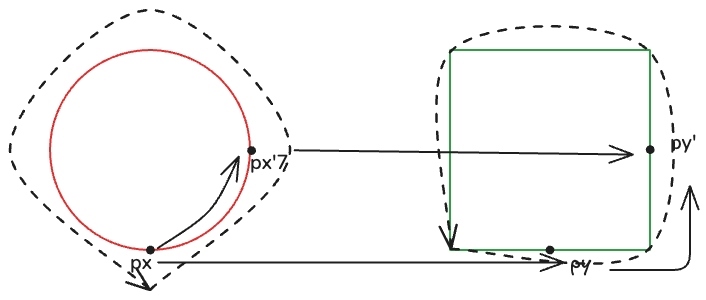
\includegraphics[width=.7\linewidth]{circle-to-square.png}

                Imagine a mapping where we go around the circle once, but around 
                the square twice. [TK] No matter how we stretch this mapping, 
                we can never get something that maps from the circle to the 
                square that go around the same number of times. The formal 
                name for this concept is a \textbf{winding number}. Thus, 
                all mappings in this setting are homotopic if they share a 
                winding number. Further more, we can group the mappings that 
                are homotopic [TK, need to explain why homotopy is an equivalence
                relation] into something known as \textbf{homotopy classes}.
            }
            \item[c] {
                Include an illustration, or plan how you will make your illustration.

                A made a rough illustration of the example above.
            }
        \end{enumerate}
    }
\end{enumerate}

\section*{Exercise 3}
\begin{itemize}
  \item Points attempted: 6
  \item Self-assessed score: 6/6.
  \item Time spent: 60 minutes.
  \item Difficulty: 4/10.
  \item Questions/Feedback: Clarity, correctness.
\end{itemize}
Let \(G\) be a group. Then we say that \(a \in G\) is conjugate to \(b \in G\) if there exists \(g \in G\) such that \(a = g b g^{-1}\). The relation is conjugate to is an equivalence relation, so it allows us to partition \(G\) into equivalence classes (which we call conjugacy classes).
Intuitively, \(a\) and \(b\) are conjugate if performing \(a\) from one perspective is the same as performing \(b\) from another perspective.
As an example, a horizontal flip and a vertical flip of a square are conjugate in \(D_4\) because if you're standing \(90^\circ\) to the right of me and I do a horizontal flip of the square, it will look like a vertical flip from your perspective—but a horizontal flip to me will never look like a \(180^\circ\) rotation to you.
In the following exercises you will be looking at conjugacy classes of the symmetry group of the hexagon.
  
\begin{enumerate}
    \item {
        Prove that \(e\) is in its own conjugacy class.

        \begin{proof}
            For all \(g \in G\), \(g e g\inv = g g\inv = e\). Therefore, \(e\) 
            is only ever conjugate to itself, thus it is its own conjugacy class.
        \end{proof}
    }

    \item {
        Find an example of \(g \in D_6\) such that \(r^2 = g r^4 g^{-1}\).
    
        Let \(g = f\). Now, we have the equation \(r^2 = f r^4 f\inv = f r^4 f = ff r^2 = r^2 \). 
    }

    \item {
        Find an example of \(g \in D_6\) such that \(f = gr^2fg\inv\).

        First, we feel that \(g\) is of the form \(r^k\). Thus, we can write the 
        equation \(f = r^k r^2 f r^{-k}\). We can use some algebra to manipulate 
        the equation to solve for \(k\), and thus \(g\). 
        \begin{align}
            f &= r^k r^2 f r^{-k} \\
            f &= r^{k+2} f r^k \\
            f &= r^{2k + 2} f \\
            r^{2k + 2} &= e \\
            2k + 2 &= 0, 6 \\
            k &= -1, 2
        \end{align}

        We see that for both \(g = r\inv = r^5\) and \(g = r^2\), \(f = g r^2f g\inv\).
    }

    \item {
        Prove that if \(\phi\colon D_6 \to H\) is a homomorphism, and \(g_1\) is conjugate to \(g_2\) in \(D_6\), then \(\phi(g_1)\) is conjugate to \(\phi(g_2)\) in \(H\).
    
        \begin{proof}
            First, we see that because \(g_1\) is conjugate to \(g_2\), there exists 
            some \(d \in D_6\) such that \(g_1 = d g_2 d\inv\). Since \(\phi\) is 
            a homomorphism, it must preserve structure.

            Therefore, 
            \begin{align}
                \phi(g_1)   &= \phi(d g_2 d\inv) \\
                            &= \phi(d) \phi(g_2) \phi(d\inv) \\
                            &= \phi(d) \phi(g_2) \phi(d)\inv \\
            \end{align}

            Since \(\phi(d) \in H\), \(\phi(g_1)\) must be conjugate to \(\phi(g_2)\).
        \end{proof}
    }

    \item {
        Prove that if \(\phi\colon D_6 \to H\) is a homomorphism, \(H\) is an abelian group, and \(g_1\) is conjugate to \(g_2\) in \(D_6\), then \(\phi(g_1) = \phi(g_2)\).

        \begin{proof}
            Following from the above proof, we have \(\phi(g_1) = h \phi(g_2) h\inv\) 
            for some \(h \in H\). Now, because \(H\) is abelian, we can rearrange 
            the RHS to be \(h h\inv \phi(g_2) = e_H \phi(g_2)\). Therefore, 
            \(\phi(g_1) = \phi(g_2)\).
        \end{proof}
    }

    \item {
        Let \(\Phi\colon D_6 \to \mathbb{Z}/2\mathbb{Z}\) be defined by \(\Phi(r) = 0\) and \(\Phi(f) = 1\), and use this to show that \(r^nf\) is not conjugate to \(r^m\) for any integers \(n\) and \(m\).
    
        First, we show that \(\Phi\) is a homomorphism by looking at the group 
        presentations of \(D_6\) and the \(\text{Im}_{\Phi}(D_6)\).

        \[D_6 = \ang{ r, f \mid r^6 = f^2 = (rf)^2 = e}\]
        \[\text{Im}_\Phi (D_6) = \ang{ 0, 1 \mid 0^6 = 1^2 = (01)^2 = e }\]

        These group presentations show that \(\Phi\) is structure preserving, 
        therefore \(\Phi\) is a homomorphism.

        Now, if \(\Phi\) is a homomorphism, then conjugacy is preserved across 
        the mapping. In other words, if \(r^n f = g r^m g\inv\), then 
        \(\Phi(r^n f) = \Phi(g) \Phi(r^m) \Phi(g)\inv\).

        Now, we use the group presentation of \(\text{Im}_\Phi (D_6)\) to simplify to 
        \[ 1 = h 0 h\inv.\]

        Because \(\Z / 2\Z\) is abelian, we have a contradiction, therefore 
        \(r^nf\) can not be conjugate to \(r^m\).
    }

    \item {
        Let \(\psi\colon D_6 \to \mathbb{Z}/2\mathbb{Z}\) be defined by \(\psi(r) = 1\) and \(\psi(f) = 0\), and use this to prove that none of the elements in \(\{r, rf, r^3, r^3f, r^5, r^5f\}\) are conjugate to any of the elements in \(\{e, f, r^2, r^2f, r^4, r^4f\}\).
    
        Similar to the previous proof, we examine the group presentation of the 
        image of \(\Phi\). 
        Notice that 
        \[\text{Im}_\Phi (D_6) = \ang{ 0, 1 \mid 1^6 = 0^2 = (01)^2 = e }\]
        shows that \(\Phi\) is a homomorphism.

        Now, let \(A = \set{r, rf, r^3, r^3f, r^5, r^5f}\), and 
        \(B = \set{e, f, r^2, r^2f, r^4, r^4f}\). Now, using the group presentation,
        notice that \(\Phi(a) = 1\) for all \(a \in A\), and \(\Phi(b) = 0\) for 
        all \(b \in B\). 0 and 1 are not conjugate in \(\Z / 2\Z\), therefore 
        none of the elements of \(A\) are conjugate to any of the elements of \(B\).
    }

    \item {
        Let \(\varphi\colon D_6 \to S_3\) be the homomorphism defined by \(\varphi(f) = (1\ 2)\) and \(\varphi(r) = (1\ 2\ 3)\). Note that \(S_3\) is not an abelian group, but use this homomorphism to show that \(r^3 \in D_6\) is in its own equivalence class.
    
        First, we see that \(\varphi(r^3) = e_{S_3}\). Since \(r^3 \in \text{ker}(\varphi)\),
        \(r^3\) must be in its own conjugacy class.
    }

    \item {
        Partition the dihedral group of the hexagon \[         D_6 = \langle r, f \mid r^6 = f^2 = (rf)^2 = e \rangle       \] into conjugacy classes. You don't have to prove every piece of this, but you do have to make a note of any claims that you made that you didn't prove.
        
        First, we showed that \(\set e\) is its own conjugacy class. 
        Similarly, \(\set{r^3}\) is its own conjugacy class. (I don't think 
        we actually proved that the elements of a kernel are in their own 
        conjugacy class).

        Then, we see see that \(A\) and \(B\) can potentially be conjugacy
        classes, but we also showed that elements of the form \(r^nf\) can not 
        be conjugate to elements of the form \(r^m\).

        Therefore, we can partition \(A\) and \(B\) into the sets:
        \(\set{r^1, r^5}, \set{r^2, r^4}, \set{f, r^2f, r^4f}, \set{rf, r^3f, r^5f}\).
    }
\end{enumerate}
  
    

\end{document}
